Le stage s'intéressant à l'implémentation d'un algorithme d'ordonnancement sur une plateforme hétérogène, une carte possédant un tel processeur est mis à ma disposition. Cette carte se nomme ROCK960 et est fabriquée par l'entreprise \textit{96Boards}. Cette carte de développement contient de nombreuses interfaces, mais nous nous contenterons d'utiliser l'interface série TTL. Nous nous connecterons à cette dernière via un convertisseur USB vers TTL. Cela permettra d'interfacer via un terminal qui fonctionnera avec une liaison série. 

 \begin{figure}[H]
    \centering
    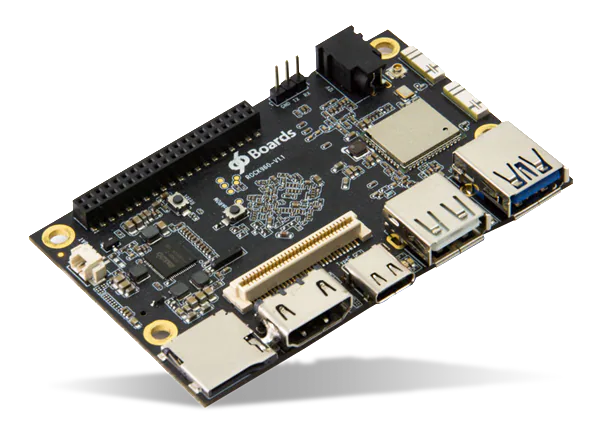
\includegraphics[width=0.75\textwidth]{Images/ROCK960.png}
    \caption{Carte ROCK960}
 \end{figure}



\subsubsection{Le processeur RK3399}
Au centre de la carte est un \gls{SoC} Rockchip RK3399. Comme le montre la figure \ref{fig:archi_rk3399}, cette puce contient entre autre deux clusters de cœurs, ou processeurs. Deux d'entre eux sont des processeurs Cortex-A72 et les quatre autres sont des processeurs Cortex-A53. Par la suite, on numérotera ces processeurs de 0 à 3 pour les A53 et 4 et 5 pour les A72. Ces 6 processeurs utilisent le même jeu d'instruction : ARMv8-A 64-bit. Cela sera important par la suite afin de faciliter la migration de tâches entre les processeurs, en effet si les jeux d'instructions des processeurs étaient différents, plusieurs copies du code compilé devraient exister tout en maintenant un lien d'équivalence entre les deux codes. Cela est bien au-delà de la portée de mon stage, mais serait un point intéressant à explorer.

\begin{figure}[H]
    \centering
    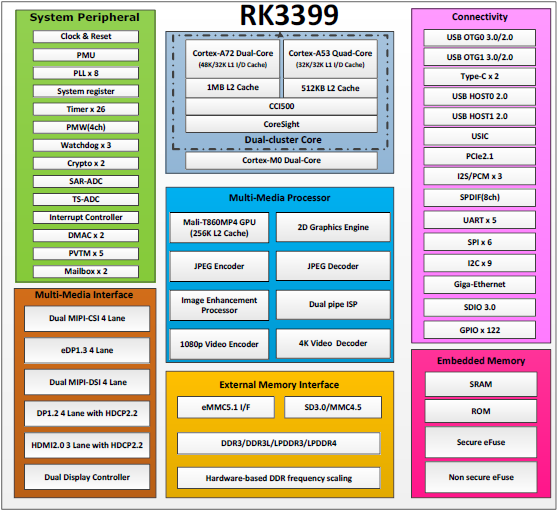
\includegraphics[width=0.45\paperwidth]{Images/RK3399_Block_Diagram.png}
    \caption{Architecture du processeur RK3399}
    \label{fig:archi_rk3399}
\end{figure}

Le SOC RK3399 contient bien d'autres composants et peut interfacer avec de nombreux périphériques (écran HDMI, USB, caméra MPI-CSI, SPI, UART, I2C, etc...) comme le montre la figure \ref{fig:archi_rk3399}. Ce diagramme nous montre aussi que les deux \gls{cluster}s de processeurs ne partagent ni les caches L1 ni les caches L2, mais sont interconnectés par une interface CCI-500 qui, selon le site des développeurs ARM, permet la cohérence des caches des deux clusters.


\subsubsection{Interfacer avec la carte}

Comme mentionné précédemment, la carte possède une sortie HDMI, mais nous nous contenterons d'utiliser l'interface série TTL. Nous nous connecterons à cette dernière via un convertisseur USB vers TTL. Cela permettra d'interfacer via un terminal qui fonctionnera avec une liaison série. J'ai utilisé l'utilitaire en ligne de commande \textit{minicom} pour me connecter à la carte. Pour que cela fonctionne, il faut configurer le \textit{baudrate} à une vitesse de 1M bauds, 8 bits de données, 1 bit de parité et 1 bit de stop (8N1).
La figure \ref{fig:terminal} montre le terminal série de \textit{minicom} connecté à la carte.


\begin{figure}[H]
    \centering
    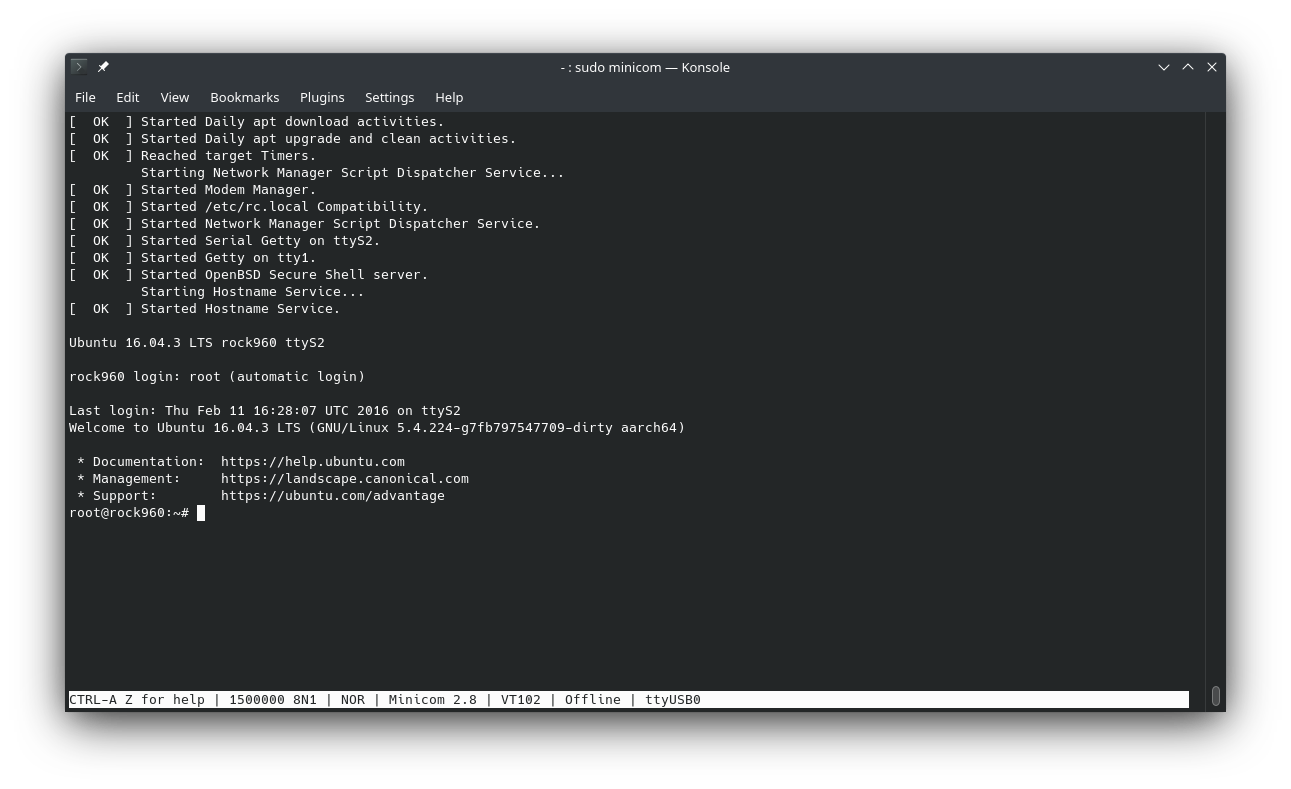
\includegraphics[width=0.75\textwidth]{Images/CaptureTerminalMinicom.png}
    \caption{Terminal série via minicom connecté à la carte}
    \label{fig:terminal}
\end{figure}

